
\documentclass[12pt,french,titlepage]{article}
\usepackage[utf8]{inputenc}
\usepackage{babel}
\usepackage[T1]{fontenc}
\usepackage{mathtools}
\usepackage{amssymb}
\usepackage{amsthm}
\usepackage{amsmath}
\usepackage{hyperref}
\usepackage{graphicx}
\usepackage{float}
\usepackage[dvipsnames]{xcolor}
\definecolor{darkWhite}{rgb}{0.94,0.94,0.94}
\usepackage{tcolorbox,listings}
\usepackage{vmargin}
\lstset{
  aboveskip=3mm,
  belowskip=-2mm,
  backgroundcolor=\color{darkWhite},
  basicstyle=\footnotesize,
  breakatwhitespace=false,
  breaklines=true,
  captionpos=bc,
  commentstyle=\color{ForestGreen},
  deletekeywords={...},
  escapeinside={\%*}{*)},
  extendedchars=true,
  keepspaces=true,
  keywordstyle=\color{blue},
  language=C,
  literate=
  {²}{{\textsuperscript{2}}}1
  {⁴}{{\textsuperscript{4}}}1
  {⁶}{{\textsuperscript{6}}}1
  {⁸}{{\textsuperscript{8}}}1
  {€}{{\euro{}}}1
  {é}{{\'e}}1
  {è}{{\`{e}}}1
  {ê}{{\^{e}}}1
  {ë}{{\¨{e}}}1
  {É}{{\'{E}}}1
  {Ê}{{\^{E}}}1
  {û}{{\^{u}}}1
  {ù}{{\`{u}}}1
  {â}{{\^{a}}}1
  {à}{{\`{a}}}1
  {á}{{\'{a}}}1
  {ã}{{\~{a}}}1
  {Á}{{\'{A}}}1
  {Â}{{\^{A}}}1
  {Ã}{{\~{A}}}1
  {ç}{{\c{c}}}1
  {Ç}{{\c{C}}}1
  {õ}{{\~{o}}}1
  {ó}{{\'{o}}}1
  {ô}{{\^{o}}}1
  {Õ}{{\~{O}}}1
  {Ó}{{\'{O}}}1
  {Ô}{{\^{O}}}1
  {î}{{\^{i}}}1
  {Î}{{\^{I}}}1
  {í}{{\'{i}}}1
  {Í}{{\~{Í}}}1,
  %morekeywords={*,...},
  numbers=left,
  numbersep=10pt,
  numberstyle=\tiny\color{black},
  rulecolor=\color{black},
  showspaces=false,
  showstringspaces=false,
  showtabs=false,
  stepnumber=1,
  stringstyle=\color{gray},
  tabsize=4,
  title=\lstname,
}
\lstdefinestyle{frameStyle}{
    basicstyle=\footnotesize,
    numbers=left,
    numbersep=20pt,
    numberstyle=\tiny\color{black}
}
 
\tcbuselibrary{listings,skins,breakable}
 
\newtcbinputlisting{\cinput}[2][]{
    arc=0mm,
    top=0mm,
    bottom=1mm,
    left=3mm,
    right=0mm,
    width=\textwidth,
    %listing engine=listings,
    listing file={#2},
    listing only,
    listing options={style=frameStyle},
    breakable
}
 

\title{Etude de cas - Collège.}
\medskip

\author{Salmân Abibou \& Rodrigo Ferreira Rodrigues\& Eldis Ymeraj \\ \hline
Université Clermont Auvergne\\ \hline}
\vfill

\date{\today}

\begin{document}
	\maketitle


	\tableofcontents
	\newpage
	
	\section{Etude sémantique du texte}
	
	\subsection{Polysèmes}
	
	\begin{itemize}
	    \item \textbf{Cours}          --> cours que l'on peut assimiler à des séances et les cours dans le sens matière.
	    \item  \textbf{Liste}          --> Liste des éleves et liste des matériels.
	    \item \textbf{Classe}  --> Classe de 6è et par niveau superieur.
	    \item \textbf{Salle} --> Salle de classe, salles machine, salle de sport et salle de cours.
	    \item \textbf{Capacité} --> Capacité de laboratoires et capacité de Salles Machines.
	    \item \textbf{Nom de famille} --> Nom de famille des élèves et nom de famille des responsables légaux.	
	    \item \textbf{Prénom}--> Nom de famille des élèves et nom de famille des responsables légaux.
	    \item \textbf{Séance} --> Seance type, seance exeptionelle et seance normale.
	    \item \textbf{Date} --> Date de séance exceptionelle et date de la séance type.
	    \item \textbf{Matériel} -> matériel prêtable et matériel déjà présent dans la salle
	  \end{itemize}
	  
	  \subsection{Synonymes}
	  
	  \begin{itemize}
	      \item Seance et Cours
	      \item Responsables légaux et parents
	      \item Eleve et Etudiant
	      \item Niveau et Classe
	      \item Document type listant les élèves absents  et fiche
	      \item Intervention et Matière
	  \end{itemize}
	  
	  \subsection{Choix}
	  
	  \begin{itemize}
	      \item \textbf{Séance} : une séance correspond à un cours
	      \item \textbf{Classe} : désigne l'ensemble des élèves assistants aux mêmes séances 
	  \end{itemize}
	  
	  \section{DCC}
	  
	  \begin{figure}[H]
	      \centering
	      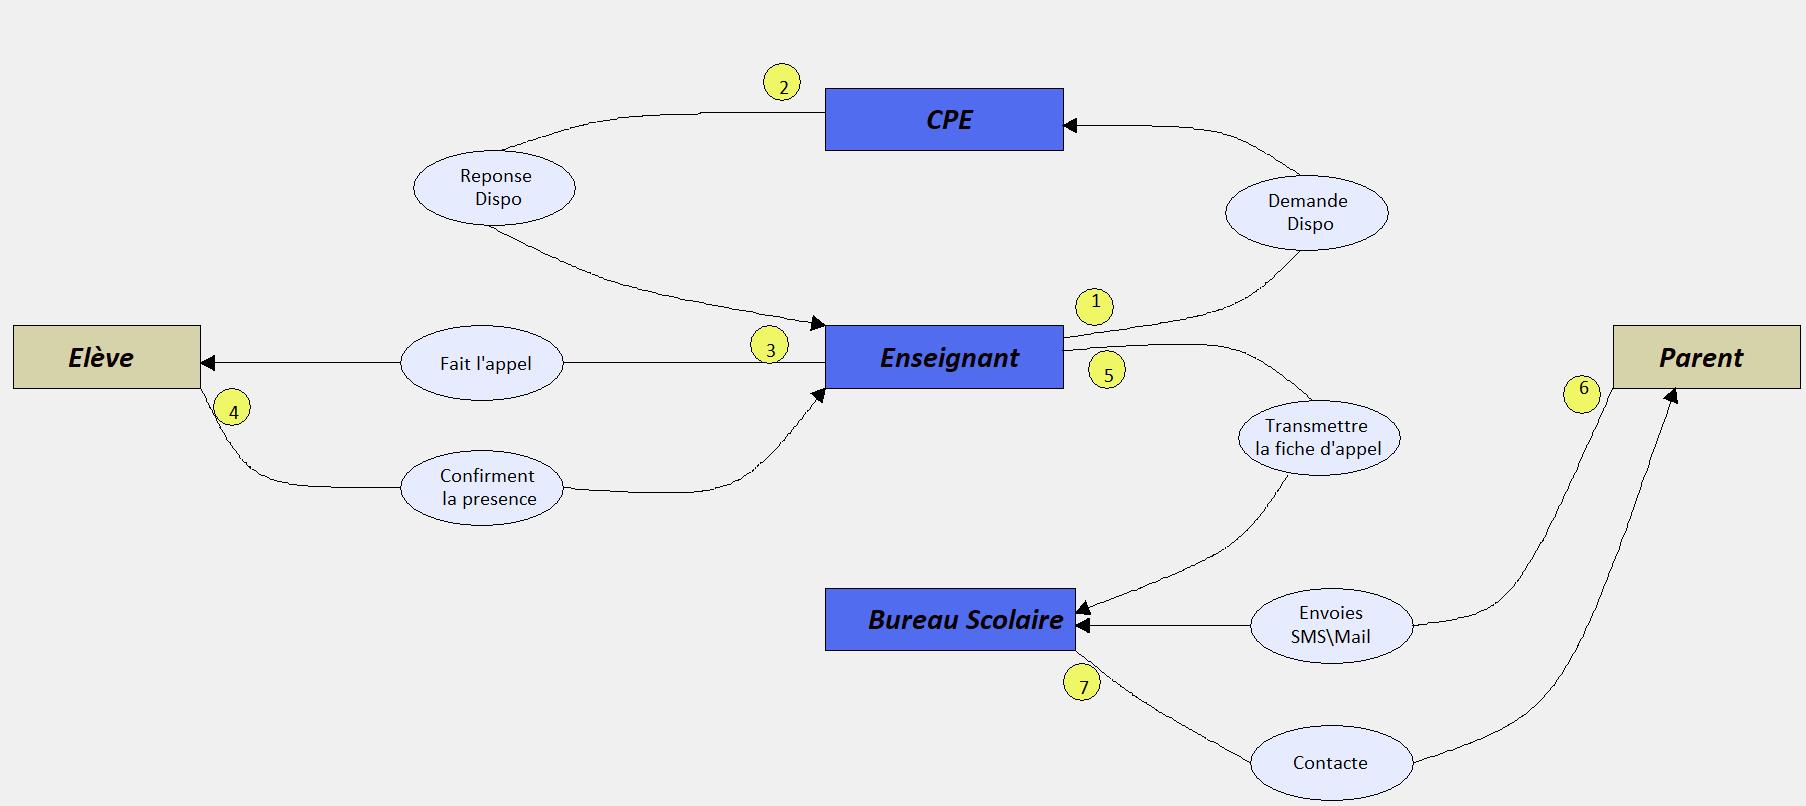
\includegraphics[scale=0.35]{./DCC.jpg}
	      \caption{DCC}
	  \end{figure}
	  
	  \section{Dictionnaire de données}
	  
	  \begin{tabular}{|p{4cm}|p{3cm}|p{1cm}|p{1cm}|p{1cm}|p{2cm}|}
	  \hline
	      Code Rubrique & Libellé & Type &Nature & Calcul & Contrainte d'intégrité \\ \hline
	      \hline
	       capacité	& Capacité de la salle &	N &	E	& * & *	\\ \hline 
dateDebutCreneau &	Date du début du créneau &	Date &	E & * &		Un créneau ne peut pas débuter à 12h\\ \hline
dateOrigine &	Date à laquelle devait se tenir originellement la séance &	Date &	E & * & *\\ \hline	
dateReport &	Date à laquelle est reportée la séance &	Date &	E & * &*		\\ \hline
debutAbsence &	Date du debut de l'absence	Date &	E &	* & * &*	\\ \hline
demiGroupe	& Numéro du demi-groupe &	N &	E & * & *		\\ \hline
emailParent &	Adresse mail du représentant légal & AN &	E & * & *	\\ \hline	
finAbsence &	Fin de l'absence &	Date &	E & * & * 	\\ \hline
heureCreneau &	Heure à laquelle se déroule le créneau &	Heure &	E & * & *	\\ \hline	
heureDebutCreneau &	Heure du début du creneau &	Heure &	E & * & *	\\ \hline	
idAbsence &	Numéro de l'absence &	N &	E & * & *		\\ \hline
idCreneau &	Numéro du créneau &	N &	E & * & *		\\ \hline
idSéance &	Numéro de la séance	& N &	E & * & *		\\ \hline
idSeanceExcep	& Numéro de la séance exceptionnelle &	N &	E & * & *	\\ \hline	
idSurv	& Identifiant du Surveillant &	N &	E & * & *	\\ \hline	
jourCreneau	& Jour de la semaine où se déroule le créneau &	A &	E & * & *	\\ \hline	
justificatif	& Justificatif de l'absence	& A &	E &  & 	\\ \hline
matière	& Nom de la matière	& A &	E &  & 	\\ \hline

	  \end{tabular}
	  
	  \begin{tabular}{|p{4cm}|p{3cm}|p{1cm}|p{1cm}|p{1cm}|p{2cm}|}
	       nomEleve &	Nom de famille de l'élève &	A &	E &	* &	* \\ \hline
nomMatériel	& Nom du matériel &	A &	E & &		\\ \hline
NomParent &	Nom de famille du responsable légal &	A &	E	& &	\\ \hline
numClasse &	Numéro de classe &	AN &	E	& &	\\ \hline
numEleve &	Numéro de l'élève &	N &	E &	* &	XXXXXXXXX\\ \hline
numEnseignant &	Numéro de l'enseignant &	N &	E & &		\\ \hline
numMatPrêtable &	Numéro du matériel prêtable &	N &	E & &	\\ \hline	
numMatSalle &	Numéro du matériel présent dans la salle &	N &	E & &	\\ \hline	
numSalle &	Numéro de la salle &	N &	E & &		\\ \hline
numTelParent &	Numéro de téléphone des parents &	N &	E & &	\\ \hline	
prénomElève &	Prénom de l'élève &	A &	E & &		\\ \hline
raisonReport &	Raison du report de la séance &	A &	E & &	\\ \hline	
semaine &	Type de semaine &	A &	E & & A ou B		\\ \hline
sexeParent &	Sexe du responsable légal &	A &	E & &	\\ \hline	
TypeContactPref &	Moyen de contact préférentiel du responsable légal &	A &	E & &	\\ \hline	
typeDeSéance &	Type de cours &	A &	E & & cours, TD ou TP		\\ \hline
typeSalle &	Type de salle &	A &	E & & Labo, machine, sport, classique		\\ 
\hline
	  \end{tabular}
	  
	  \section{Dependances fonctionnelles symetriques}
	  
Etant donne que emailParent et numTelParent peuvent identifier le parent/representant legal, on a emailParent $\rightarrow$ numTelParent et numTelParent $\rightarrow$ emailParent. Dans la suite de notre travail nous allons identifier le parent avec emailParent.
	  
	  \section{Dépendances fonctionnelles}
	  
	  On obtient la liste de dépendances fonctionnelles  élémentaires directes non-réflexives à but
      simple :
      
      \begin{enumerate}
          \item numEleve $\rightarrow$ nomEleve  
\item	numEleve $\rightarrow$ prénomEleve   
\item numEleve	$\rightarrow$ demiGroupe   

\item numSalle $\rightarrow$ capacité    
\item	numSalle $\rightarrow$ typeSalle   

\item emailParent $\rightarrow$ numTelParent   
\item	   emailParent $\rightarrow$ sexeParent    
\item	   emailParent $\rightarrow$ nomParent	   
\item emailParent $\rightarrow$ typeContactPref   

\item idAbsence $\rightarrow$ numEleve    
\item	 idAbsence $\rightarrow$ debutAbsence   
\item	 idAbsence $\rightarrow$ finAbsence  

\item numMatSalle $\rightarrow$ numSalle   
	\item   numMatSalle $\rightarrow$ nomMatériel 

\item numMatPrêtable $\rightarrow$ nomMatériel

\item demiGroupe $\rightarrow$ numClasse   

\item idSeance $\rightarrow$ numEnseignant   
\item	idSeance $\rightarrow$ numSalle    
\item	idSeance $\rightarrow$ matiere    
\item	idSeance $\rightarrow$ idCreneau   
\item	idSeance $\rightarrow$ typeCours    

\item idSeanceExcep $\rightarrow$ idSeance   
\item	     idSeanceExcep $\rightarrow$ dateReport   
\item	     idSeanceExcep $\rightarrow$ raisonReport   
\item	     idSeanceExcep $\rightarrow$ dateOrigine    

\item idCreneau $\rightarrow$ jourCreneau   
\item	 idCreneau $\rightarrow$ heureCreneau   
\item	 idCreneau $\rightarrow$ semaine  

\item idAbsence $\rightarrow$ justificatif
      \end{enumerate}
      
      \subsection{Graphe}
      
      \subsection{Rubriques identifiantes}
      
      On distingue les rubriques identifiantes suivantes :
      
      \begin{itemize}
          \item numEleve
          \item numSalle
          \item emailParent
          \item idAbsence
          \item nomMatériel
          \item numMatSalle
          \item numMatPrêtable
          \item idSéance
          \item idSéanceExcep
          \item idCréneau
          \item numClasse
          \item demiGroupe
          \item numSurv
          
      \end{itemize}

    \subsection{Tableau des DF}
    
    \begin{tabular}{|p{4cm}|p{5cm}|p{5cm}|}
    \hline
        DF simple /cible identifiante & Oui & Non\\
        \hline
        Oui &  3, 10, 13, 14, 15, 16, 18, 20, 22  
        & 1, 2, 4, 5, 6, 7, 8, 9, 11, 12, 17, 19, 21, 23, 24, 25, 26, 27, 28, 29 \\
         \hline
        Non & & \\
        \hline
        
        
    \end{tabular}

	    
	   \section{Ebauches}
	   
	   \subsection{MCD}
	   On obtient le MCD suivant :
    \begin{figure}[H]
	      \centering
	      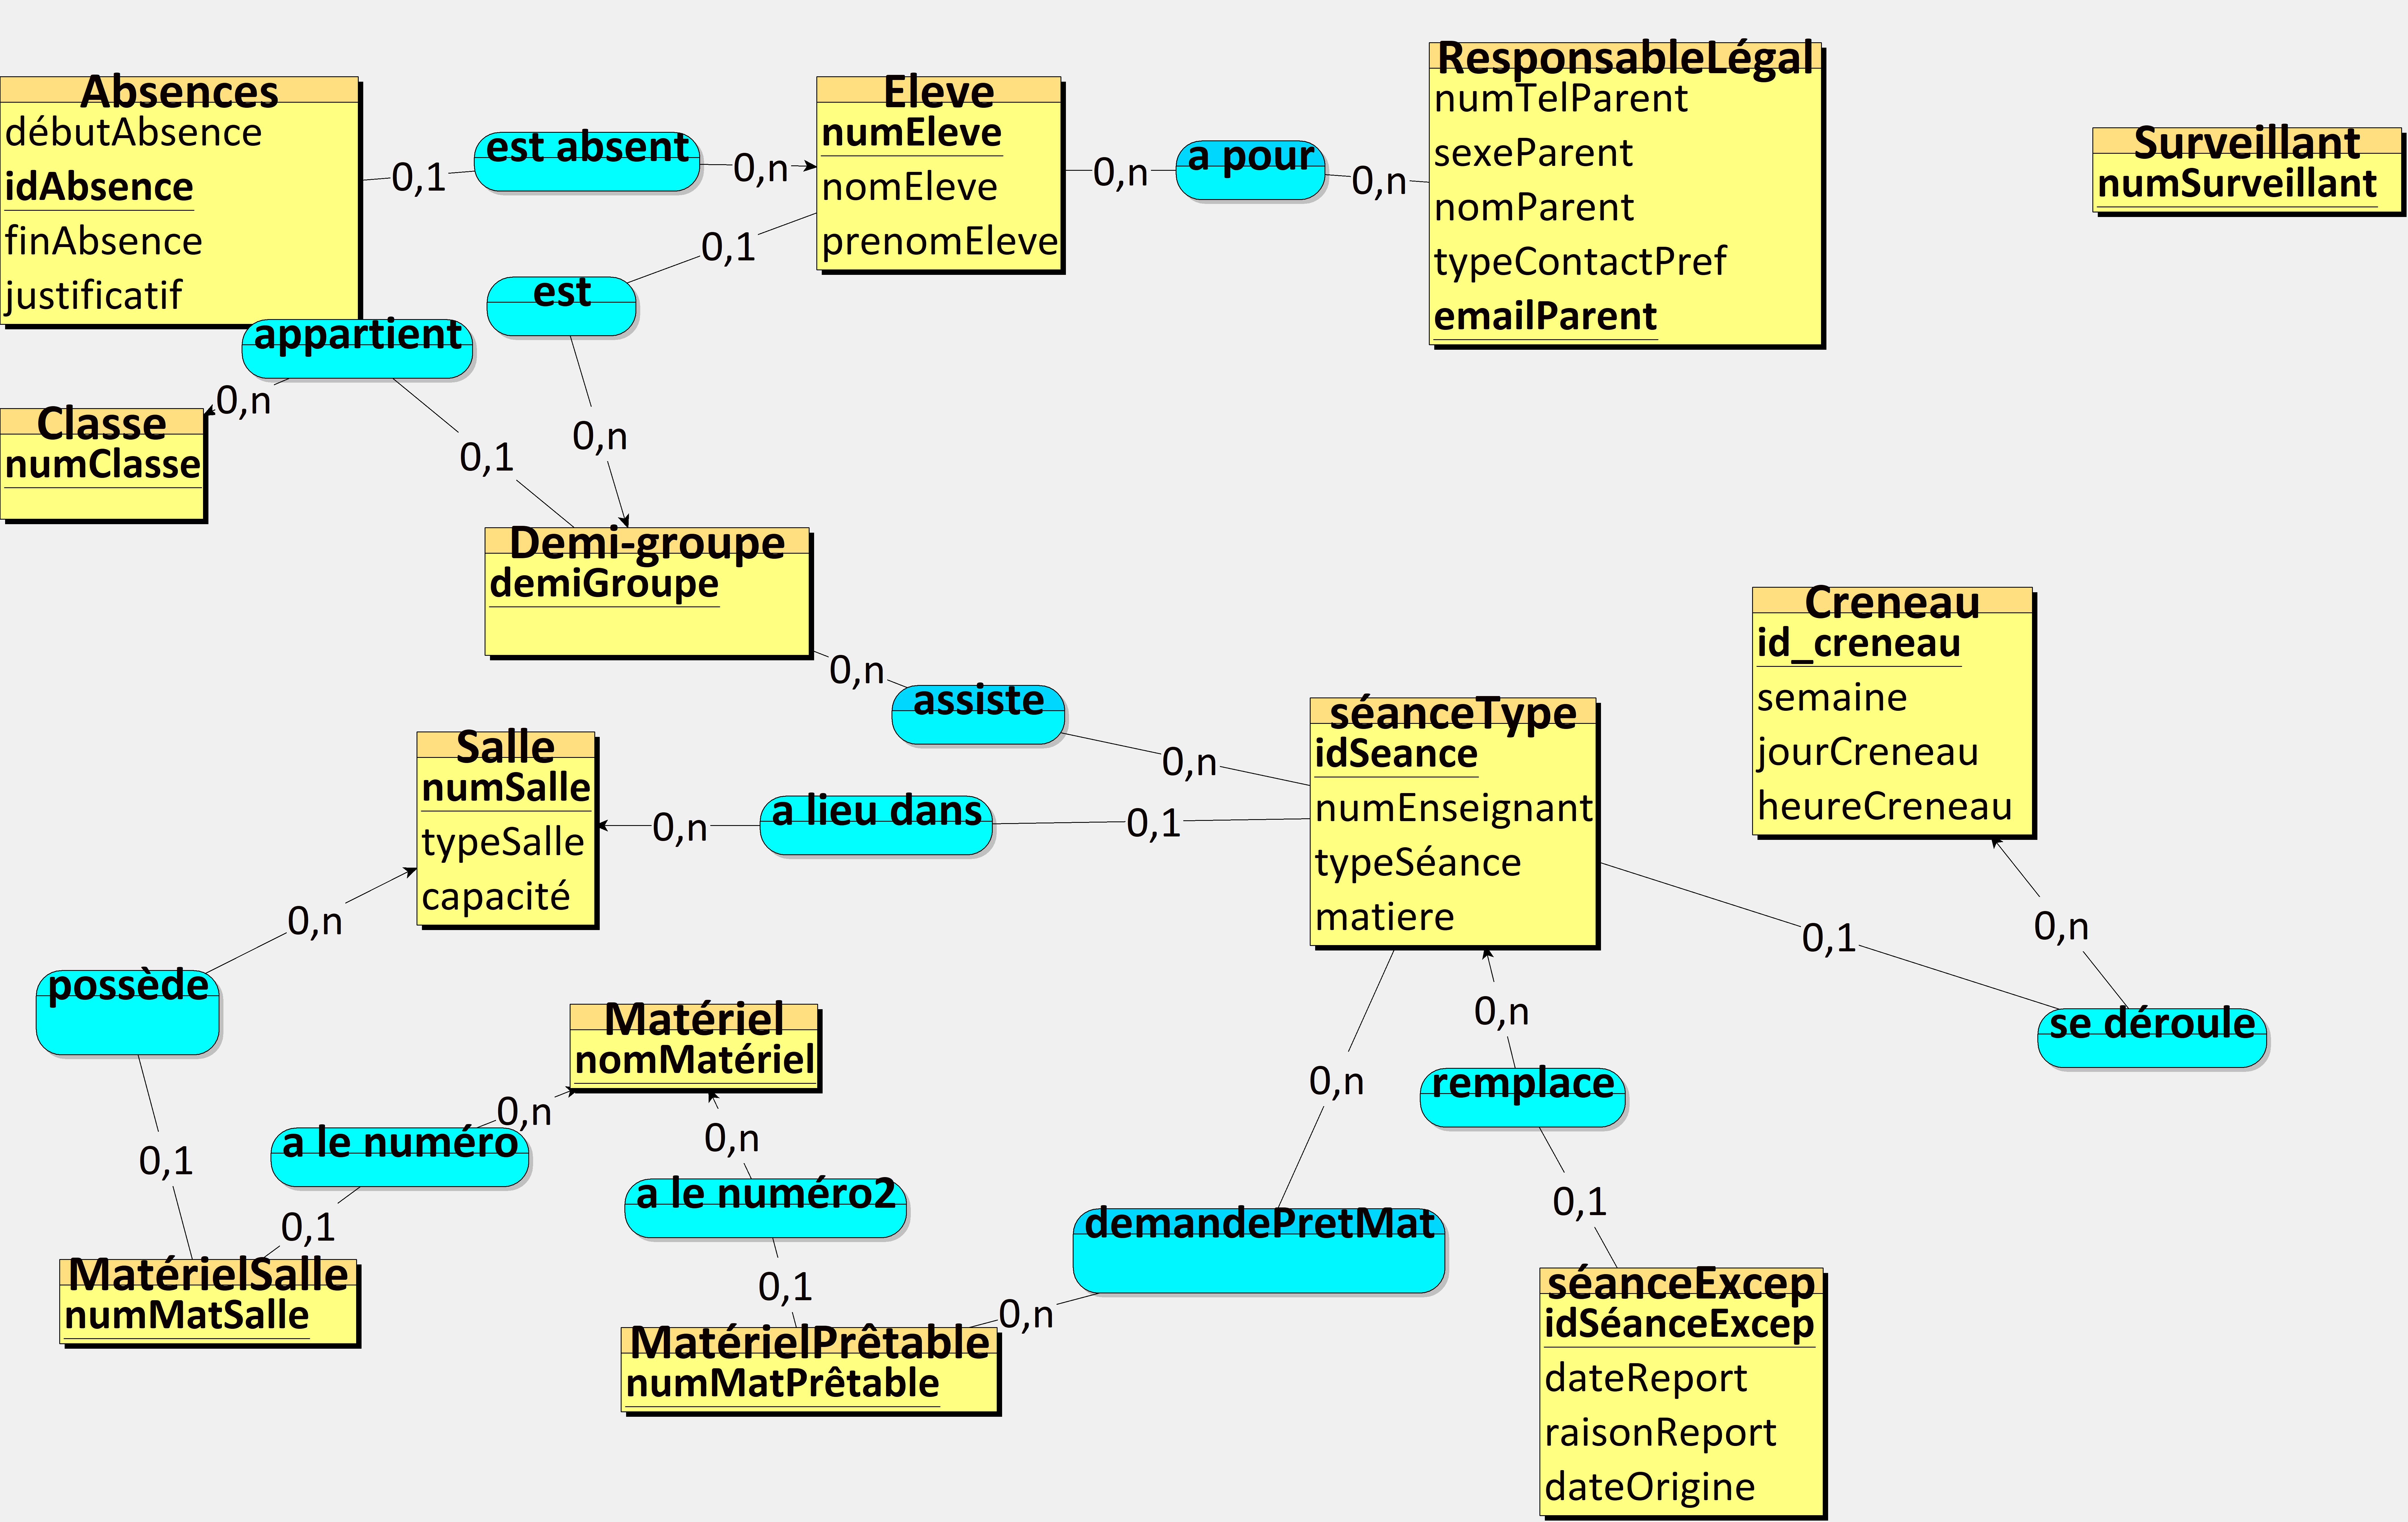
\includegraphics[scale=0.08]{./ebauche_mcd.jpg}
	      \caption{Ebauche du MCD}
	      
	   
	      
	  \end{figure}
	  
	  \subsection{MLD}
	  
	  On obtient le MLD suivant :

    \begin{figure}[H]
	      \centering
	      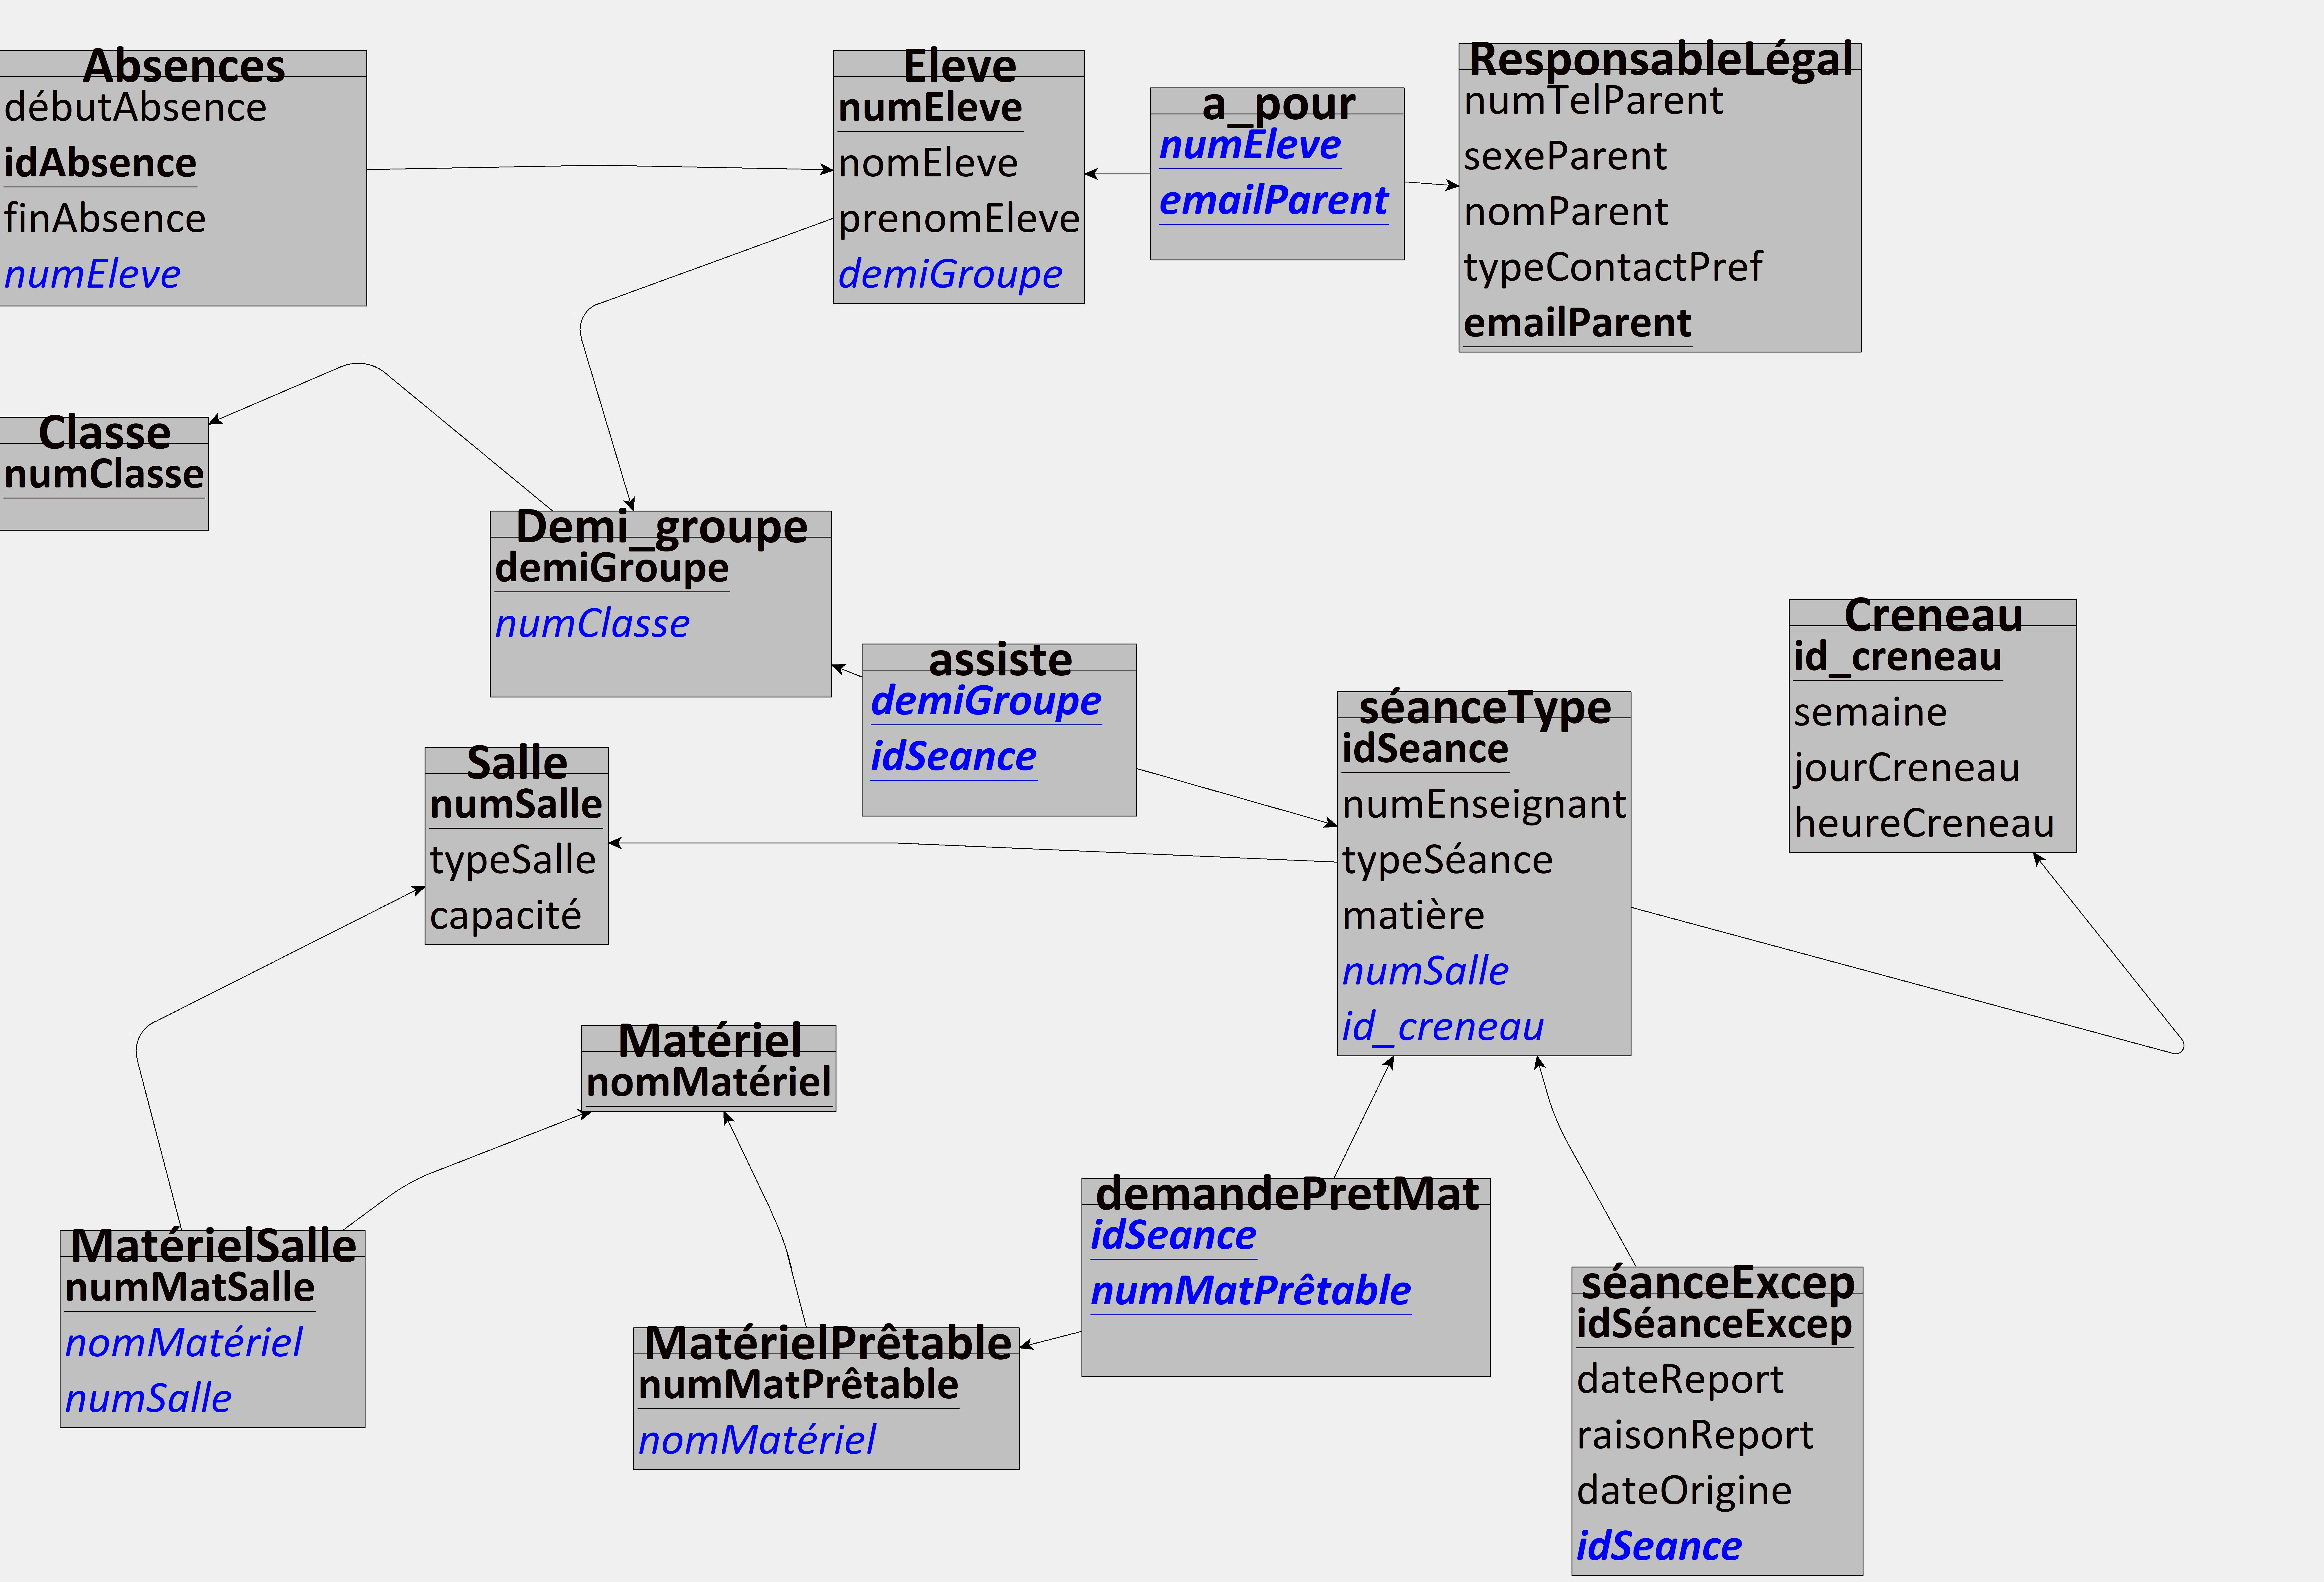
\includegraphics[scale=0.08]{./ebauche_mld.jpg}
	      \caption{MLD obtenu à partir de l'ébauche de MCD}
	      
	   
	      
	  \end{figure}
    
    \section{Aménagement}
    
    \subsection{MCD}
    
    \begin{figure}[H]
	      \centering
	      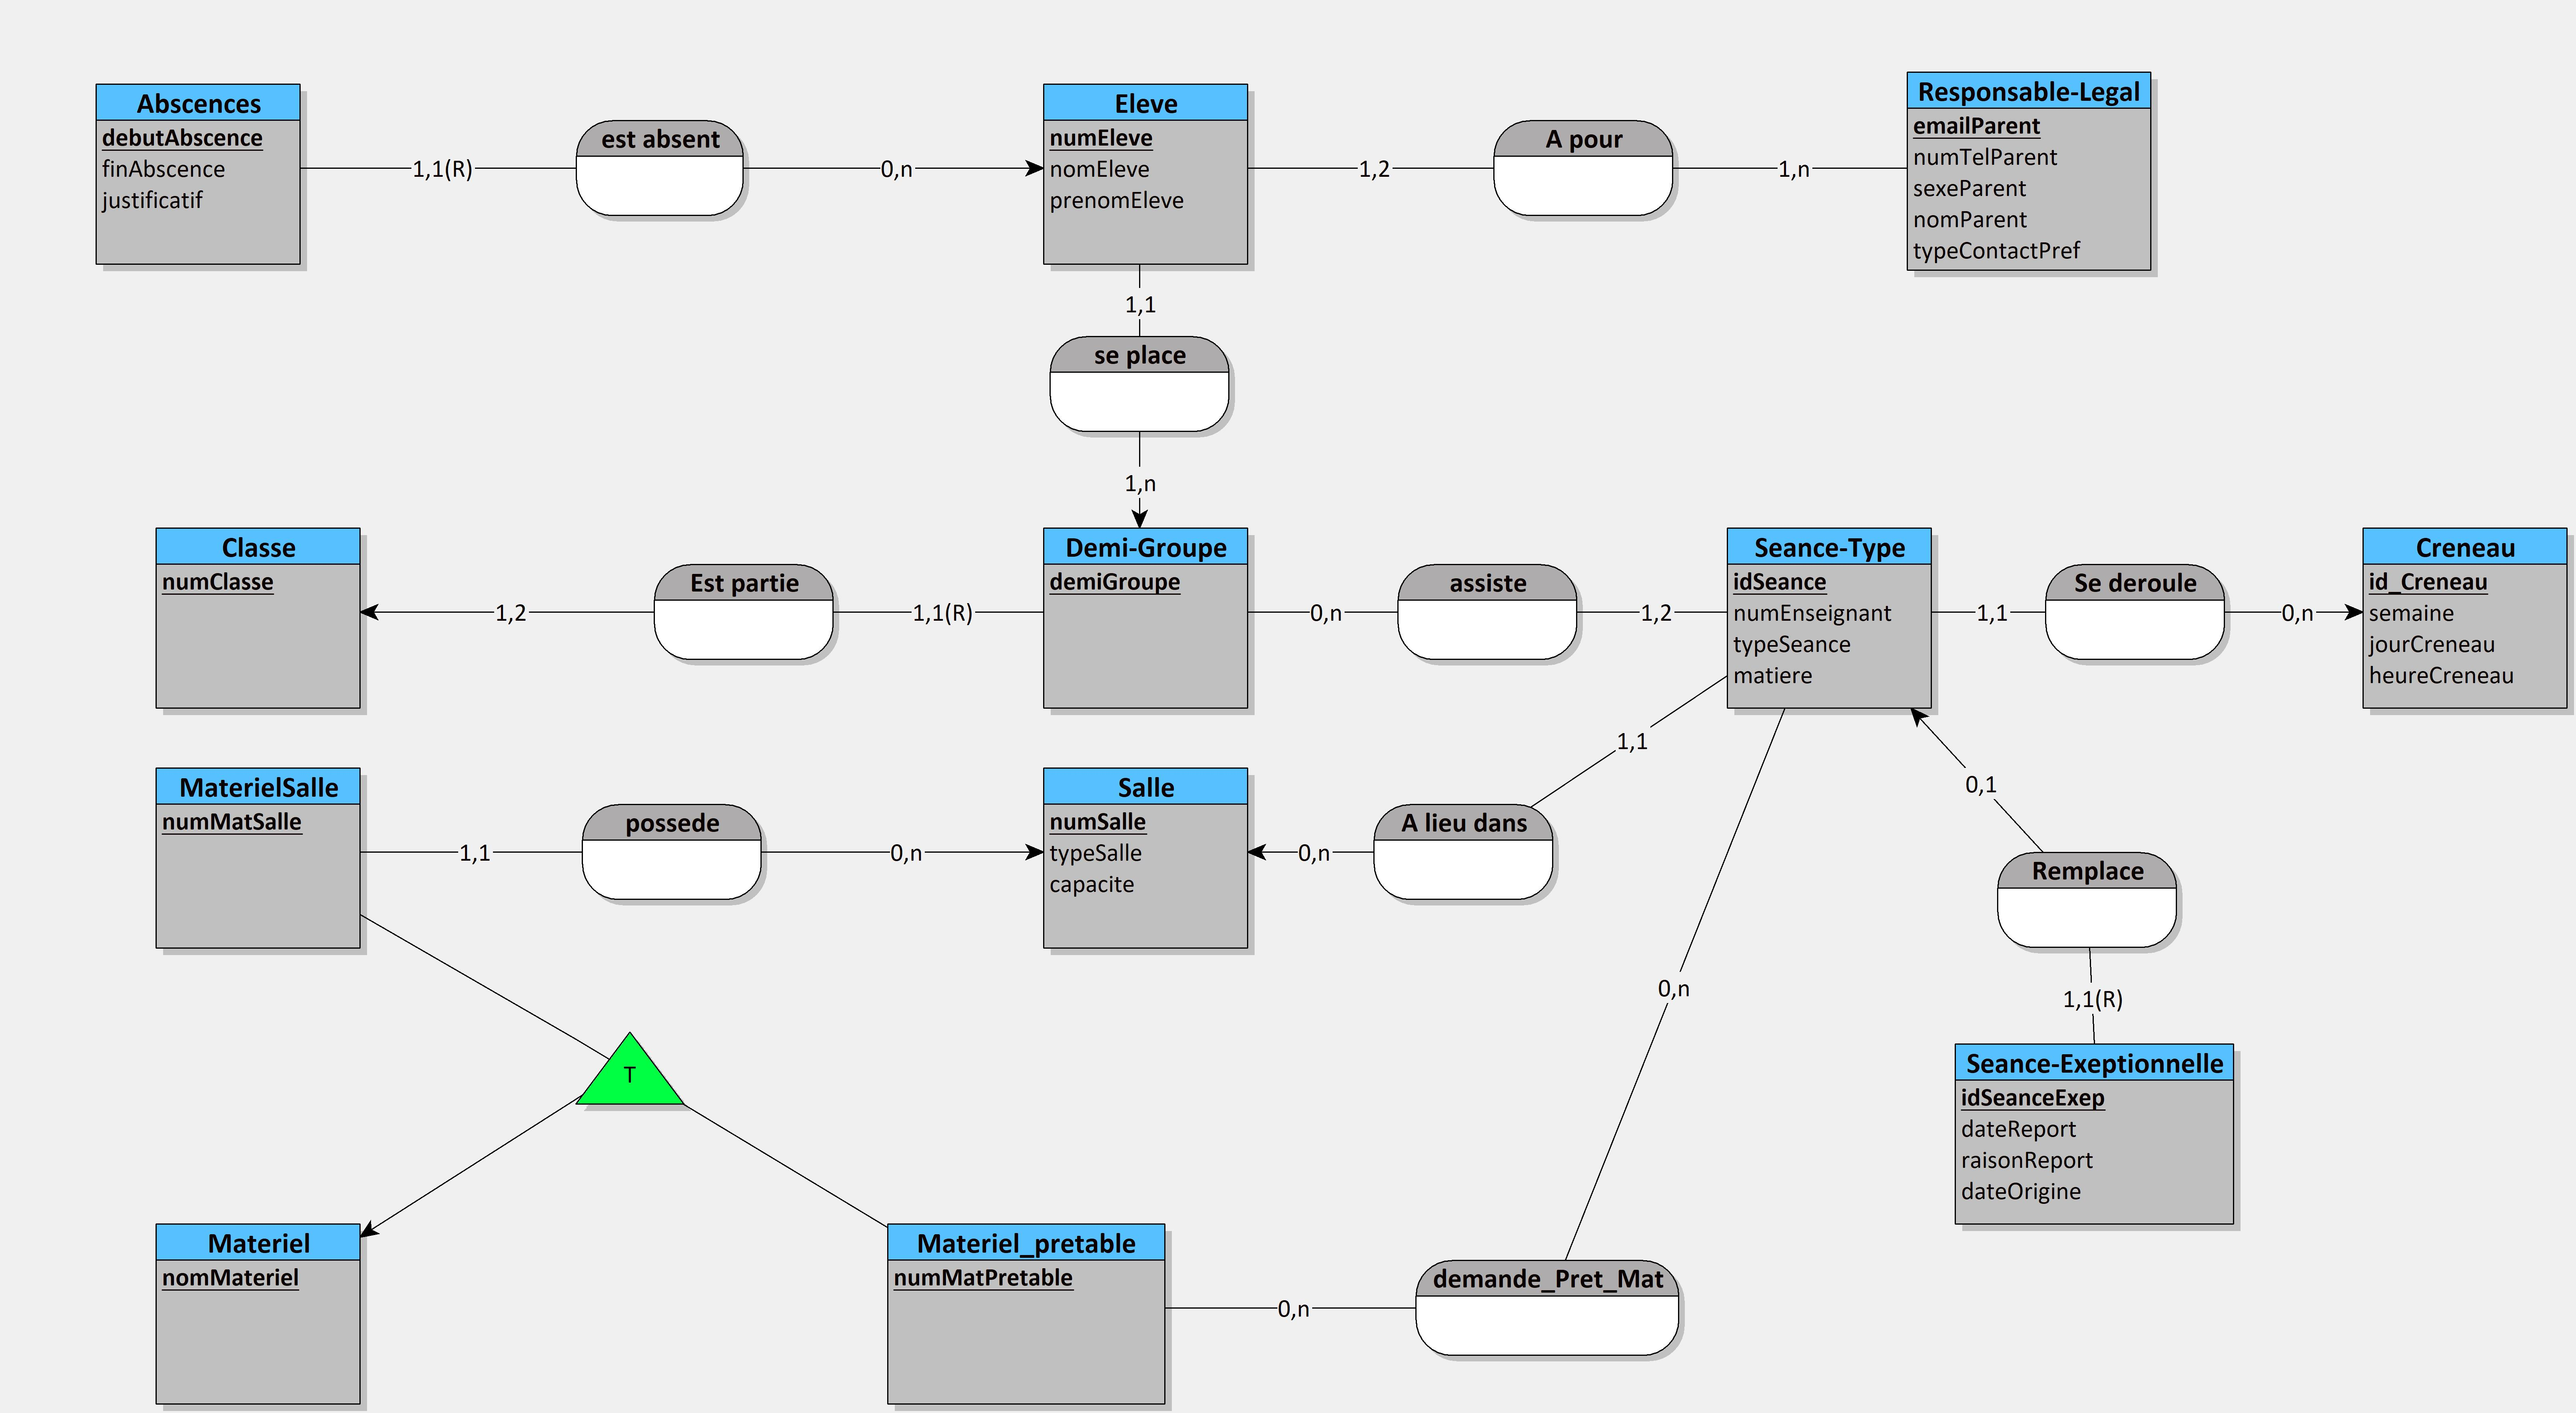
\includegraphics[scale=0.08]{./mcd_amenage.jpg}
	      \caption{MCD aménagé}
	      
	   
	      
	  \end{figure}
	  
	  \subsection{Explications des aménagements}
	  
	  \begin{itemize}
	      \item implémentation d'un héritage pour décrire le cas des matériaux
	  \end{itemize}
	  
	  \subsection{MLD}
	  
	  \begin{figure}[H]
	      \centering
	      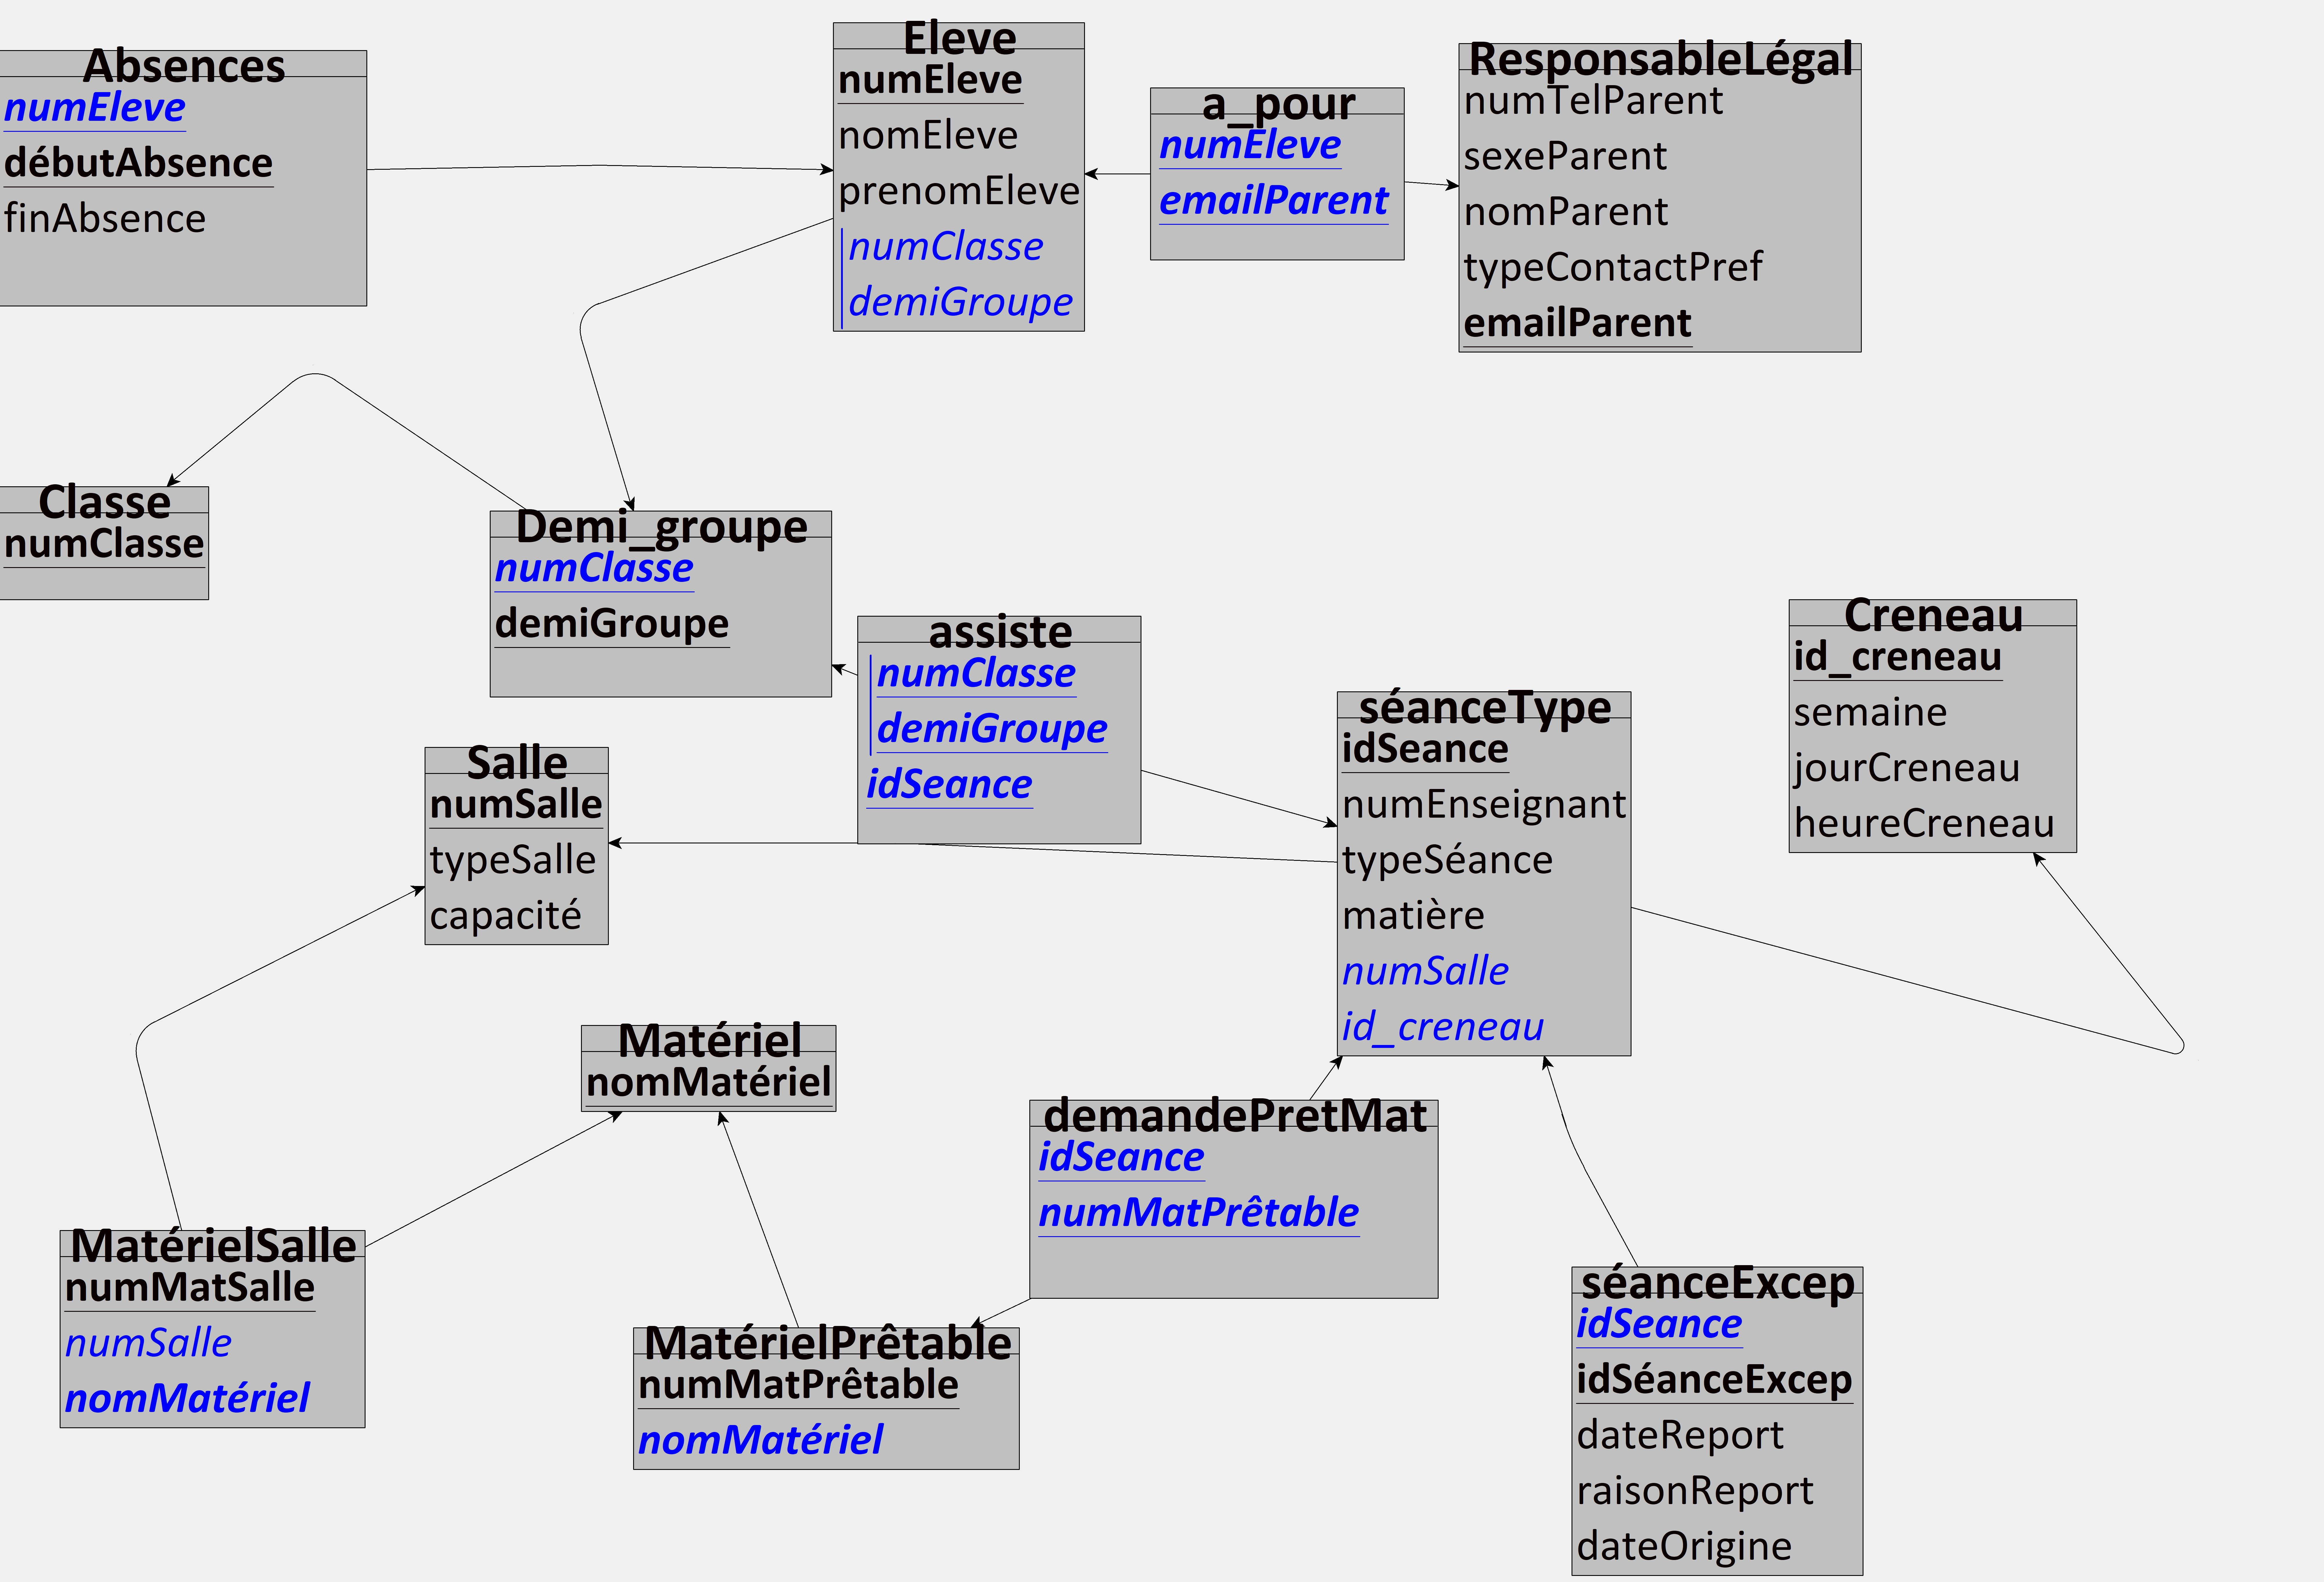
\includegraphics[scale=0.08]{./mld_amenage.jpg}
	      \caption{MLD obtenu à partir du MCD aménagé}
	      
	   
	      
	  \end{figure}
	  
	  \section{Scripts SQL}
	  
	  \lstinputlisting[language=SQL, firstline=1, lastline=126, frame=trBL, caption = Scripts SQL obtenus]{scripts_sql.txt}
	  
	  \section{Conclusion}
    

	
	
	
\end{document}

